\chapter{局域量子场与一维狄拉克方程}

我们已经通过量子场的量子、产生和湮灭算符，以及非相对论粒子的最简单哈密顿量接触过量子场。现在我们要让这套机器真正运转起来。首先，我们将看到——而不仅仅是断言——空间局域的哈密顿量如何守恒动量。然后，我们将让场的乘积描述散射和衰变，并观察哈密顿量的反复作用如何生成图解微扰论的雏形。只有在这之后，我们才会转向所承诺的费米子问题。最干净的入口还不是费米子场，而是一维狄拉克方程。

\section{再论场哈密顿量}

将一种非相对论粒子的哈密顿量写为
\begin{equation}
H_0=\int dx\,
\psi^\dagger(x)
\left[-\frac{\partial_x^2}{2m}+V(x)\right]
\psi(x).
\label{eq:l9-nonrel-hamiltonian}
\end{equation}
记号看起来是一维的，但开头的论证中没有任何东西依赖于这一限制：在三维中，\(x\)可以代表矢量\(\mathbf{x}\)，\(dx\)可以代表\(d^3x\)，而\(-\partial_x^2\)可以代表\(-\nabla^2\)。

算符\(\psi^\dagger(x)\)在\(x\)处产生一个粒子，而\(\psi(x)\)在彼处湮灭一个粒子。它们的正规序乘积
\begin{equation}
n(x)=\psi^\dagger(x)\psi(x)
\end{equation}
就是局域数密度。因此势能项读作
\begin{equation}
H_V=\int dx\,V(x)n(x).
\end{equation}
这正是我们为经典气体所写下的：数出\(x\)附近的粒子，给每个粒子赋予势能\(V(x)\)，然后对空间求和。在这个阶段，粒子之间并不相互作用。它们可以对外部施加的势作出响应，但除此之外哈密顿量是独立单粒子能量之和。

先简化再逆转方向是有益的。取势为常数，\(V(x)=V_0\)。常数势不施加任何力，但其算符含义是透明的：
\begin{equation}
\begin{aligned}
H_V&=V_0\int dx\,\psi^\dagger(x)\psi(x)=V_0N,\\
N&=\int dx\,n(x).
\end{aligned}
\end{equation}
它给每个粒子相同的附加能量。为了在非相对论描述中保留静止能量，选择\(V_0=mc^2\)。该项随后为每个粒子计入一份静止能量。我们保留这个本来乏味的常数，因为它保持平移不变性，并使数数操作变得可见。

\section{哈密顿量作为更新规则}

说动量守恒是什么意思？我们应当用哈密顿量做了什么来表述答案。为了避免把\(\psi\)同时用于场算符、单粒子波函数和多体态，把多体态称为\(\lvert\Phi(t)\rangle\)。在短时间间隔\(\epsilon\)内，
\begin{equation}
\lvert\Phi(t+\epsilon)\rangle
=\left(1-i\epsilon H+O(\epsilon^2)\right)
\lvert\Phi(t)\rangle,
\label{eq:l9-short-update}
\end{equation}
其中\(\hbar=1\)。不变的状态是第一项；第一阶修正由\(H\)生成。迭代这个更新就得到Schr\"odinger方程。

动量守恒现在有了具体的含义。如果初始态具有确定的总动量\(P\)，那么\(H\lvert\Phi\rangle\)必须具有相同的总动量。其他性质可能改变，单个粒子可能交换动量，但哈密顿量不能把状态带入总\(P\)不同的扇区。我们可以通过在动量基中重写哈密顿量来直接检验这一点。

\section{空间积分作为动量{\proseunicodefont δ}函数}

选择傅里叶约定
\begin{align}
\psi(x)&=\int\frac{dp}{\sqrt{2\pi}}\,a(p)e^{ipx},\\
\psi^\dagger(x)&=\int\frac{dq}{\sqrt{2\pi}}\,a^\dagger(q)e^{-iqx}.
\label{eq:l9-field-fourier}
\end{align}
算符\(a(p)\)湮灭一个动量为\(p\)的粒子。算符\(a^\dagger(q)\)产生一个动量为\(q\)的粒子。不同的字母是必要的：这两个动量独立积分，直到空间积分将它们联系起来。

从数项开始：
\begin{align}
N
&=\int dx\,\psi^\dagger(x)\psi(x)\\
&=\int\frac{dp\,dq}{2\pi}\,
a^\dagger(q)a(p)
\int dx\,e^{i(p-q)x}.
\end{align}
剩余的积分为
\begin{equation}
\int dx\,e^{i(p-q)x}=2\pi\delta(p-q).
\end{equation}
对于\(p\ne q\)，相位振荡并在正负贡献之间抵消。对于\(p=q\)，它完全不振荡。狄拉克{\proseunicodefont δ}分布正是把这两个事实结合起来的精确对象。因此，
\begin{align}
N
&=\int dp\,dq\,a^\dagger(q)a(p)\delta(p-q)\\
&=\int dp\,a^\dagger(p)a(p).
\label{eq:l9-number-momentum}
\end{align}
该算符移除一个动量为\(p\)的粒子，并放回一个动量完全相同的粒子。决定性的要素是对\(x\)的积分：它产生了{\proseunicodefont δ}函数，强制进入的动量与出去的动量相等。

\begin{classroomqa}
\lecturetimestamp{00:17:02}
\audiencequestion{当\(p=q\)时出现的无穷大怎么样了？}
\lecturerresponse{{\proseunicodefont δ}函数不是通过求其高度来使用的。它是通过积分定义的分布：\(\int dk\,\delta(k)f(k)=f(0)\)。``无限高且无限窄''这个说法只是提醒我们它的积分权重为一。在这里，它指示我们令\(p-q=0\)，于是不再留下无穷大的答案。}
\end{classroomqa}

同样的机制适用于更一般的局域单项式。假设某一项包含若干个湮灭场和若干个产生场，也许属于不同的种类，但都在同一点取值并对该点积分：
\begin{equation}
\int dx\,
\prod_{r=1}^{n} \psi_{i_r}^\dagger(x)
\prod_{s=1}^{m} \psi_{j_s}(x).
\end{equation}
设被湮灭的粒子携带动量\(p_s\)，被产生的粒子携带动量\(q_r\)。傅里叶展开给出
\begin{equation}
\int dx\,
e^{i(\sum_s p_s-\sum_r q_r)x}
=2\pi\,
\delta\!\left(\sum_s p_s-\sum_r q_r\right).
\label{eq:l9-total-momentum-delta}
\end{equation}
结果并不把\(p_1\)与\(q_1\)配对、\(p_2\)与\(q_2\)配对，等等。它只强加
\begin{equation}
\sum_{\mathrm{annihilated}}p
=
\sum_{\mathrm{created}}q.
\end{equation}
这正是相互作用所要求的规则：单个动量可以改变，但总动量不变。更深刻的表述是平移不变性。一个局域密度若在每一点以相同权重积分，就没有优先的原点，其傅里叶变换携带相应的动量守恒{\proseunicodefont δ}函数。

\begin{classroomqa}
\lecturetimestamp{00:23:04}
\audiencequestion{所提出的哈密顿量项真的是所有这些场算符的乘积吗？我们为什么要写出这样的乘积？}
\lecturerresponse{是的。这个乘积指定了在一点上哪些粒子被移除、哪些被产生。它的物理动机将来自观测到的散射或衰变过程；先建立动量论证，是为了让这些相互作用可以立即被读出。}
\end{classroomqa}

\section{动量空间与位置空间中的动能}

现在把同样的机制应用于导数项。导数作用在平面波上：
\begin{equation}
-\partial_x^2 e^{ipx}=p^2e^{ipx}.
\end{equation}
因此
\begin{align}
H_{\mathrm{kin}}
&=\int dx\,\psi^\dagger(x)
\left(-\frac{\partial_x^2}{2m}\right)\psi(x)\\
&=\int dp\,\frac{p^2}{2m}\,a^\dagger(p)a(p).
\label{eq:l9-kinetic-momentum}
\end{align}
空间积分再次强制入射与出射动量相等。新的因子\(p^2/2m\)只是用该模式的动能对每个动量模式中的粒子数加权。

\begin{classroomqa}
\lecturetimestamp{00:24:46}
\audiencequestion{对平面波求两次导数应该给出一个负号吗？}
\lecturerresponse{是的，\(\partial_x^2e^{ipx}=-p^2e^{ipx}\)。哈密顿量已经包含补偿的负号，所以\(-\partial_x^2\)具有正本征值\(p^2\)。}
\end{classroomqa}

\begin{classroomqa}
\lecturetimestamp{00:27:20}
\audiencequestion{只有当势为常数时动能才守恒吗？}
\lecturerresponse{是的。没有依赖于位置的势时，就没有力，动能单独守恒。在非恒定外势中，动能和势能可以相互交换，而如果总哈密顿量没有显式时间依赖，则它保持守恒。}
\end{classroomqa}

\begin{classroomqa}
\lecturetimestamp{00:27:42}
\audiencequestion{\(\psi^\dagger\psi\)在动量空间动能哈密顿量中的作用是什么？}
\lecturerresponse{它是计数算符。模式乘积\(a^\dagger(p)a(p)\)计数动量为\(p\)的粒子，而因子\(p^2/2m\)给每一个粒子赋予相应的动能。}
\end{classroomqa}

还有第二种方式看出正定性。分部积分一次并忽略边界项，得到
\begin{align}
\int dx\,\psi^\dagger(-\partial_x^2)\psi
&=\int dx\,(\partial_x\psi^\dagger)(\partial_x\psi).
\label{eq:l9-positive-kinetic}
\end{align}
对于在无穷远处适当消失的场，或者在周期边界条件下，边界贡献为零。结果具有绝对平方的形式，并且是非负的。它还展示出场论中常见的一种模式：能量包含场的空间导数的平方。

\section{局域接触相互作用}

现在让我们给场的乘积一个物理任务。考虑两种粒子，我们只为了保持图像熟悉而称它们为电子和质子。目前它们是被故意虚构的：两者都用玻色子算符处理，并且省略了它们真实的库仑相互作用。它们的自由哈密顿量为
\begin{equation}
H_0=\int dx\left[
\psi_e^\dagger\left(-\frac{\partial_x^2}{2m_e}\right)\psi_e
+
\psi_p^\dagger\left(-\frac{\partial_x^2}{2m_p}\right)\psi_p
\right].
\end{equation}
加上模型相互作用
\begin{equation}
H_{\mathrm{contact}}
=g\int dx\,
\psi_e^\dagger(x)\psi_p^\dagger(x)
\psi_e(x)\psi_p(x).
\label{eq:l9-contact}
\end{equation}
从右向左读。它在同一点\(x\)寻找一个电子和一个质子，湮灭它们，并在该点重新产生两者。如果两个粒子不在一起，这个局域项给出零。如果它们的worldline相交，它可以改变它们的单个动量而保持总动量不变。因此它充当一个理想化的零程散射势。

\begin{figure}[htbp]
\centering
\includegraphics[width=0.94\linewidth]{lecture_09_frame_02.png}
\caption{黑板上的接触相互作用。四个局域场算符出现在时空草图上方；相遇点是理想化相互作用唯一作用的地方。}
\lectureframe{00:35:36}
\end{figure}

\begin{figure}[htbp]
\centering
\begin{tikzpicture}[x=1.2cm,y=1.0cm,>=Latex]
\draw[->] (-3.0,0) -- (3.0,0) node[right] {$x$};
\draw[->] (0,-0.2) -- (0,4.2) node[above] {$t$};
\coordinate (v) at (0,2.0);
\fill (v) circle (1.8pt);
\draw[thick,->] (-2.2,0.4) -- (v);
\draw[thick,->] (2.0,0.4) -- (v);
\draw[thick,->] (v) -- (-1.6,3.7);
\draw[thick,->] (v) -- (2.2,3.7);
\node[left] at (-1.65,0.7) {$e$};
\node[right] at (1.55,0.7) {$p$};
\node[left] at (-1.15,3.3) {$e$};
\node[right] at (1.65,3.3) {$p$};
\node[right] at (0.12,2.05) {$g$};
\end{tikzpicture}
\caption{对局域散射图像的清晰重构。该顶点是式~\eqref{eq:l9-contact}中算符的简写，而不是经典碰撞定律。}
\end{figure}

真实的电子和质子通过库仑势在远距离上相互作用。接触模型只是最初的一小步：如果实验表明两种粒子只有在重叠时才散射，那么式~\eqref{eq:l9-contact}就是我们会放入哈密顿量的那种项。

\begin{classroomqa}
\lecturetimestamp{00:35:40}
\audiencequestion{如果能量不变，为什么这个散射算符是哈密顿量的一部分？}
\lecturerresponse{哈密顿量既是能量算符，也是改变状态的生成元。两个粒子之间的势能会在时间演化中产生散射。总能量守恒并不意味着状态或粒子各自的动量保持不变。}
\end{classroomqa}

这给出了一条实用规则。首先从实验了解粒子能够经历哪些局域过程。然后把这些过程编码进更新状态的算符中。场的乘积不是装饰性的代数：其中的带剑号因子和不带剑号因子规定了哪些粒子种类出现和消失。

\section{衰变、逆过程与厄米性}

假设气泡室显示出一条粒子种类\(A\)的径迹终止于一点，从该点射出\(B\)和\(C\)的径迹。局域过程是
\begin{equation}
A\longrightarrow B+C.
\end{equation}
执行它的算符是
\begin{equation}
V=g\int dx\,
\psi_B^\dagger(x)\psi_C^\dagger(x)\psi_A(x).
\label{eq:l9-decay-half}
\end{equation}
湮灭场移除\(A\)；两个产生场在同一点产生\(B\)和\(C\)。对每个\(x\)以相同权重积分表达了空间平移不变性，并立即给出
\begin{equation}
p_A=p_B+p_C.
\end{equation}

哈密顿量必须是厄米的。这正是使\(e^{-itH}\)为幺正并保持总概率的原因。式~\eqref{eq:l9-decay-half}本身不是厄米的，所以我们必须加上它的伴随：
\begin{equation}
H_{\mathrm{int}}
=\int dx\left[
g\,\psi_B^\dagger\psi_C^\dagger\psi_A
+g^*\,\psi_A^\dagger\psi_C\psi_B
\right](x).
\label{eq:l9-hermitian-vertex}
\end{equation}
对于实耦合\(g\)，两个系数相同。厄米共轭既交换带剑号和不带剑号的场，也反转算符顺序。在这个玻色子玩具模型中，不同种类的场对易，所以这种反转不会造成额外的复杂性。

第二项执行逆过程，
\begin{equation}
B+C\longrightarrow A.
\end{equation}
因此，一个允许该衰变的闭合幺正哈密顿量也包含复合振幅。这并不保证对于每一组选定的外部动量两个方向都会发生；能量和其他守恒定律可能使一个方向在运动学上不可达。它说的是算符及其伴随都属于动力学。

\begin{classroomqa}
\lecturetimestamp{00:42:48}
\audiencequestion{逆过程也被允许这条规则可以有例外吗？}
\lecturerresponse{在厄米闭合系统哈密顿量的层面上没有例外：伴随相互作用是必需的。某个特定的逆反应仍然可能被运动学或另一个守恒量子数所禁止，但共轭矩阵元是存在的。}
\end{classroomqa}

数\(g\)是耦合常数。如果\(g\)很小，相遇的粒子只微弱地相互作用；如果它很大，跃迁振幅就更大。耦合通常是实验中测得的参数，尽管对称性可以把几个表面上不同的耦合联系起来。

同样的语法可以处理更复杂的反应。在{\proseunicodefont β}衰变中，
\begin{equation}
n\longrightarrow p+e^-+\bar\nu_e,
\end{equation}
一个示意性的局域项包含四个场：一个湮灭中子，三个产生质子、电子和电子反中微子，再加上厄米共轭过程。这足以看出，一小组算符单项式如何开始定义量子场论。

\section{为什么哈密顿量的平方很重要}

短时公式\eqref{eq:l9-short-update}只保留到\(\epsilon\)的一阶。完整展开是
\begin{equation}
e^{-i\epsilon H}
=1-i\epsilon H-\frac{\epsilon^2}{2}H^2
+\frac{i\epsilon^3}{3!}H^3+\cdots.
\label{eq:l9-exponential}
\end{equation}
在二阶，哈密顿量作用两次。这就是第一批复合过程图像的代数起源。

对于顶点\(A\leftrightarrow B+C\)，一次作用可以将\(B+C\)合并为\(A\)，而第二次作用可以将该\(A\)重新分裂回\(B+C\)：
\begin{equation}
B+C\longrightarrow A\longrightarrow B+C.
\label{eq:l9-bc-scattering}
\end{equation}
净贡献是一个\(B+C\to B+C\)散射振幅。中间的\(A\)并不是额外观测到的事件；它标记的是在相互作用的两次作用之间被求和的那个态。

\begin{classroomqa}
\lecturetimestamp{00:49:54}
\audiencequestion{写出的二阶乘积中的\(C\)场是否应带一个匕首符号？}
\lecturerresponse{是的，算符顺序必须与所述序列一致。第一个顶点湮灭\(B\)和\(C\)并产生\(A\)；第二个顶点湮灭\(A\)并重新产生\(B\)和\(C\)。正确地写出相应的匕首符号即可恢复这一解释。}
\end{classroomqa}

\begin{figure}[htbp]
\centering
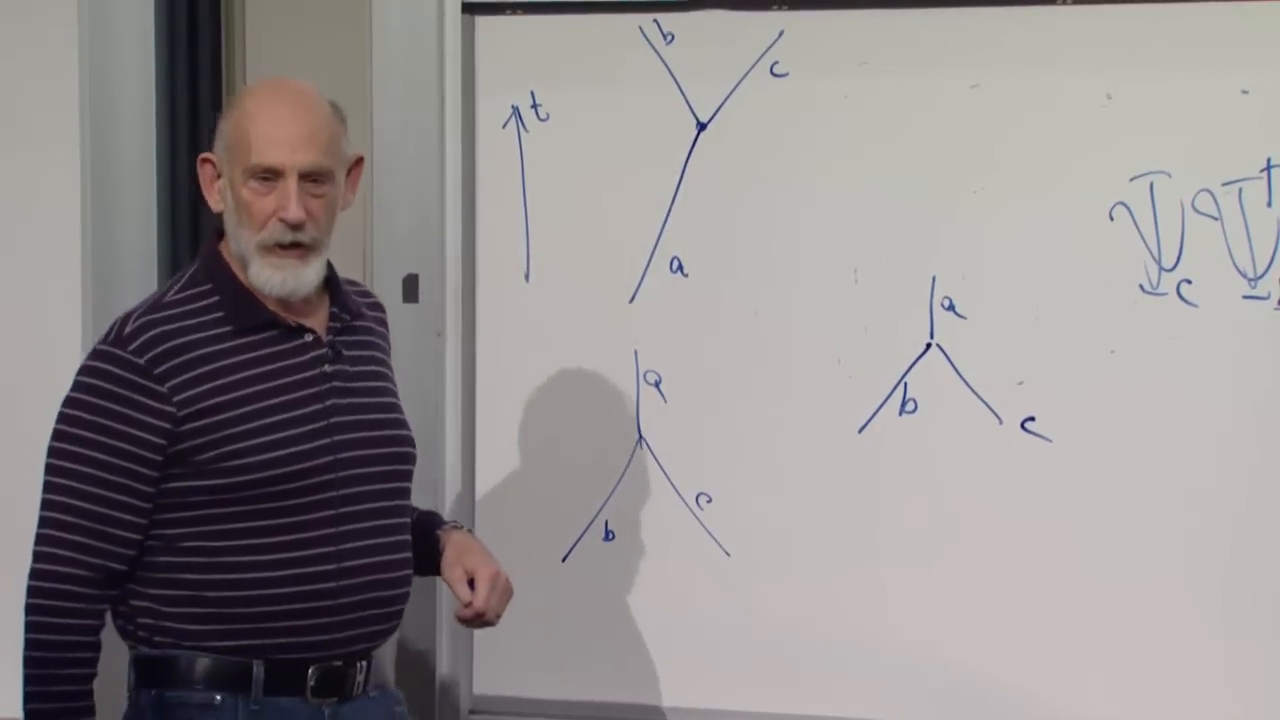
\includegraphics[width=0.94\linewidth]{lecture_09_frame_05.png}
\caption{黑板上基本\(A\leftrightarrow B+C\)顶点的两种取向。将它们并置是式~\eqref{eq:l9-bc-scattering}中二阶过程的视觉简记。}
\lectureframe{00:48:56}
\end{figure}

现在加入一个旁观者\(B\)。一次作用让\(A\)发射\(C\)并变成\(B\)；稍后的一次作用让该\(C\)与原来的\(B\)结合形成\(A\)。外线粒子仍然是\(A+B\)，但它们的动量可以改变。我们将此描述为通过交换\(C\)而发生的\(A\)与\(B\)散射。

\begin{figure}[htbp]
\centering
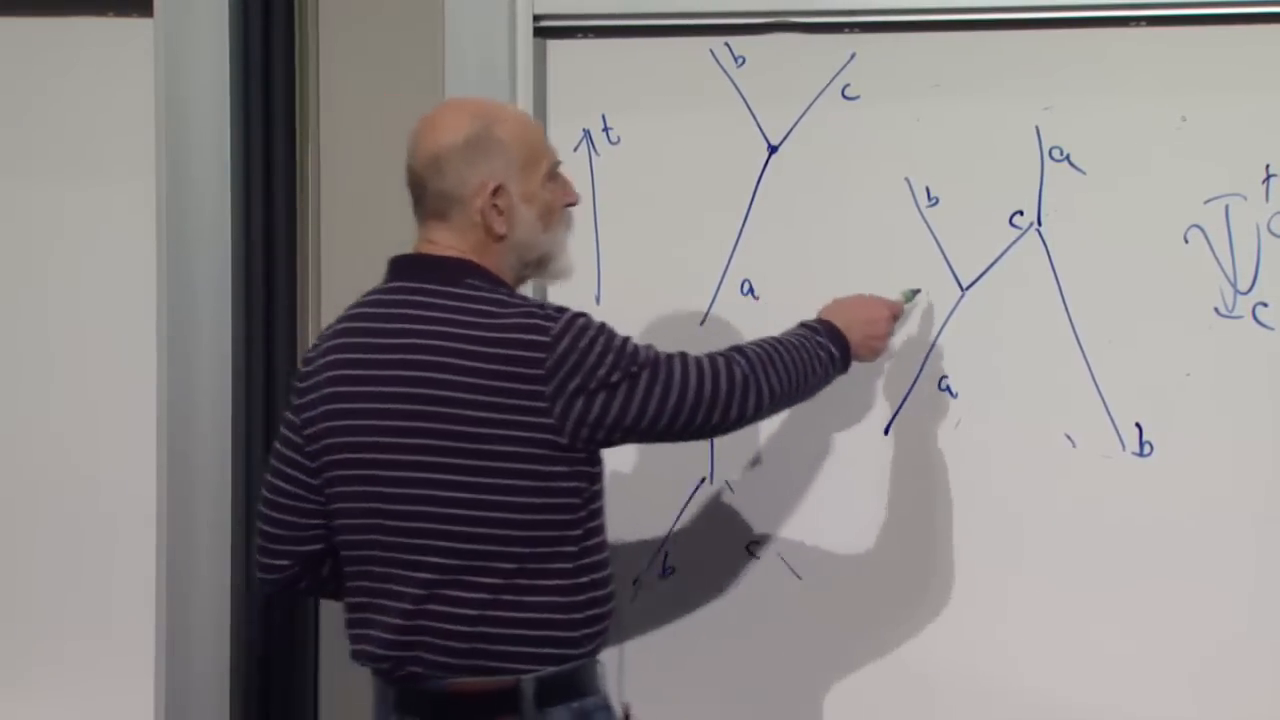
\includegraphics[width=0.94\linewidth]{lecture_09_frame_06.png}
\caption{黑板上的交换构造。右侧的图用一条内部\(C\)线连接两个基本顶点，同时外部的\(A\)和\(B\)粒子发生散射。}
\lectureframe{00:51:22}
\end{figure}

\begin{figure}[htbp]
\centering
\begin{tikzpicture}[x=1.1cm,y=1cm,>=Latex]
\draw[->] (-3.7,-0.2) -- (-3.7,4.2) node[above] {$t$};
\coordinate (v1) at (-0.9,1.25);
\coordinate (v2) at (0.9,2.95);
\fill (v1) circle (1.7pt);
\fill (v2) circle (1.7pt);
\draw[thick,->] (-2.6,0.2) -- (v1) node[midway,below left] {$A$};
\draw[thick,->] (2.6,0.2) -- (v2) node[midway,below right] {$B$};
\draw[thick,->] (v1) -- (-2.4,4.0) node[midway,left] {$B$};
\draw[thick,->] (v2) -- (2.5,4.0) node[midway,right] {$A$};
\draw[thick,->,dashed] (v1) -- (v2) node[midway,above left] {$C$};
\node[below] at (0,-0.05) {$A+B\rightarrow A+B$};
\end{tikzpicture}
\caption{对\(C\)交换的一个清晰重构。每个点贡献一个\(g\)因子，因此这个二阶项正比于\(g^2\)。}
\end{figure}

每个局域相互作用点称为一个顶点。每个顶点贡献一个其耦合常数的因子，因此双顶点贡献带有\(g^2\)，三顶点贡献带有\(g^3\)，依此类推。因此，哈密顿量中的单个项关联着一大类反应。这种经济性是量子场论如此强大的原因之一：少量局域相互作用组织起了数量庞大的散射数据。

\begin{classroomqa}
\lecturetimestamp{00:53:14}
\audiencequestion{我们把过程\(A\to B+C\to A\)称为什么？}
\lecturerresponse{它是一个自能贡献。测量到的\(A\)并不仅仅是裸的单粒子基态；相互作用态还具有附近\(B+C\)分量的振幅。对它进行散射可以揭示这种着装结构。}
\end{classroomqa}

量子电动力学提供了熟悉的例子。一个局域电子--光子顶点可以湮灭一个电子、重新产生一个电子并产生一个光子。在二阶，电子可以发射并重新吸收一个光子。人们很容易将其叙述为一部微小的电影，但其严格的意义是微扰展开中的一项。物理电子是一个包含光子分量的着装态。

课堂上关于该分量是``约百分之一''的估计传达了由精细结构常数\(\alpha_{\mathrm{em}}\simeq 1/137\)设定的尺度。光子福克分量的精确概率取决于能量分辨率以及相互作用态如何定义；它并不是孤立电子普遍具有的百分之一性质。稳健的陈述是：相互作用改变了电子可测量的结构。

\section{图能说明什么与不能说明什么}

这些图是相互作用哈密顿量幂次的计算简记。它们并不是可靠的经典历史，即粒子确定地先执行一个事件再执行另一个事件。深入内部去判定哪个中间备选``真正发生了''会改变实验并破坏相干求和，正如普通量子干涉中那样。

\begin{classroomqa}
\lecturetimestamp{00:56:52}
\audiencequestion{在第一个顶点处能量和动量都守恒吗？}
\lecturerresponse{在此处进行的等时哈密顿量构造中，空间积分立即产生一个动量{\proseunicodefont δ}函数。对于那个孤立的插入，尚未有时间积分产生能量{\proseunicodefont δ}函数。完整的时间平移不变散射振幅守恒总能量，而中间线不必满足所观测粒子的在壳关系。在协变图语言中，每个顶点处四动量守恒，但内部粒子可以离壳。}
\end{classroomqa}

朴素顶点图像中看似缺失的能量，是另一个警告：不要丢弃相互作用能。总哈密顿量并不只是自由粒子能量之和。如果产生困惑，就回到式~\eqref{eq:l9-exponential}：该图像代表的是幺正时间演化展开式中的一项。完整的费曼图技术提供了系统的时间排序、传播子、积分和对称因子，但基本物理从这里开始。

一个延伸的问题把该图理解得过于字面，将发射的光子与缓慢运动电子周围的电场相比较。

\begin{classroomqa}
\lecturetimestamp{00:58:26}
\audiencequestion{电子在某一距离处的电场，真的是由辐射光子产生的吗？这与干涉以及阿哈罗诺夫--玻姆效应如何相容？}
\lecturerresponse{静态场或感应场并不是真实辐射光子的流。量子电动力学用同一个场描述辐射和电子的电磁着装，但相应的量子态和运动学不同。对于极端相对论性电子，某些场分量可以有用地表现得像近真实光子的通量；对于缓慢电子，字面意义上的光子轨迹是错误的模型。双缝干涉和阿哈罗诺夫--玻姆效应也是非经典的场现象，但它们并不会把这个自能图变成一部机械影片。}
\end{classroomqa}

\begin{classroomqa}
\lecturetimestamp{01:01:28}
\audiencequestion{为什么该图的经典模型恰恰会失败？}
\lecturerresponse{因为计算相干地相加了所有允许的中间备选方案的振幅。经验使这些图像变得直观，但它们的字面内容从未超出定义它们的算符展开式。它们是计算\(H^2,H^3,\ldots\)的一种紧凑方式，而不是对观测到的中间事件的记录。}
\end{classroomqa}

\begin{classroomqa}
\lecturetimestamp{01:03:04}
\audiencequestion{普通的库仑相互作用能否作为光子交换的经典极限而出现？}
\lecturerresponse{能。计算适当的光子介导振幅并取非相对论静态极限，就得到库仑势。该推导比目前的算符草图更具技术性，而且仍然不应把它读作光子字面地在两个经典粒子之间跳跃。}
\end{classroomqa}

\begin{classroomqa}
\lecturetimestamp{01:03:44}
\audiencequestion{耦合常数是由场乘积计算出来的吗？}
\lecturerresponse{通常它们的数值是实验输入。对称性可以约束它们，或把本来相互独立的耦合联系起来。当这样一种关系预言了不同反应的相对强度，而实验证实了它时，这种符合尤其具有启发性。}
\end{classroomqa}

\begin{classroomqa}
\lecturetimestamp{01:04:48}
\audiencequestion{偶然对称性与规范对称性相比，作用是什么？}
\lecturerresponse{规范对称性直接约束允许的结构以及耦合之间的关系。偶然对称性并非在基本层面上被强加，而是因为所有低阶允许的相互作用恰好都尊重它才出现。它仍然可以有重要后果，尽管其起源和稳健性与规范对称性不同。}
\end{classroomqa}

非相对论场论暂时讲到这里就够了。我们承诺过要讲费米子。与其立即对它们做二次量子化，我们不如先理解它们的场算符必须满足的相对论性单粒子方程。

\section{为什么电子需要相对论}

从一维空间开始。这不是一个现实的限制，但它去掉了三维自旋的几何复杂性，同时保留了本质的代数。电子足够轻，以至于即使在原子中相对论也很重要。在氢原子中，其特征速度的量级为
\begin{equation}
v\sim\alpha_{\mathrm{em}}c\approx 0.007c,
\end{equation}
大约是光速的百分之一。对于重原子中的内层电子，粗略尺度变为\(v\sim Z\alpha_{\mathrm{em}}c\)，因此相对论修正可能相当大。无论决定性的动机来自历史好奇心还是原子精度，一个相对论性的类Schr\"odinger方程在物理上都是必要的。

通常的量子化方案从能量与动量之间的经典关系出发。非相对论地，
\begin{equation}
E=\frac{p^2}{2m},
\end{equation}
而代换
\begin{equation}
E\mapsto i\partial_t,
\qquad
p\mapsto-i\partial_x
\end{equation}
给出
\begin{equation}
i\partial_t\varphi(x,t)
=-\frac{1}{2m}\partial_x^2\varphi(x,t).
\end{equation}

相对论则给出，取\(c=1\)，
\begin{equation}
E^2=p^2+m^2.
\label{eq:l9-rel-dispersion}
\end{equation}

\begin{figure}[htbp]
\centering
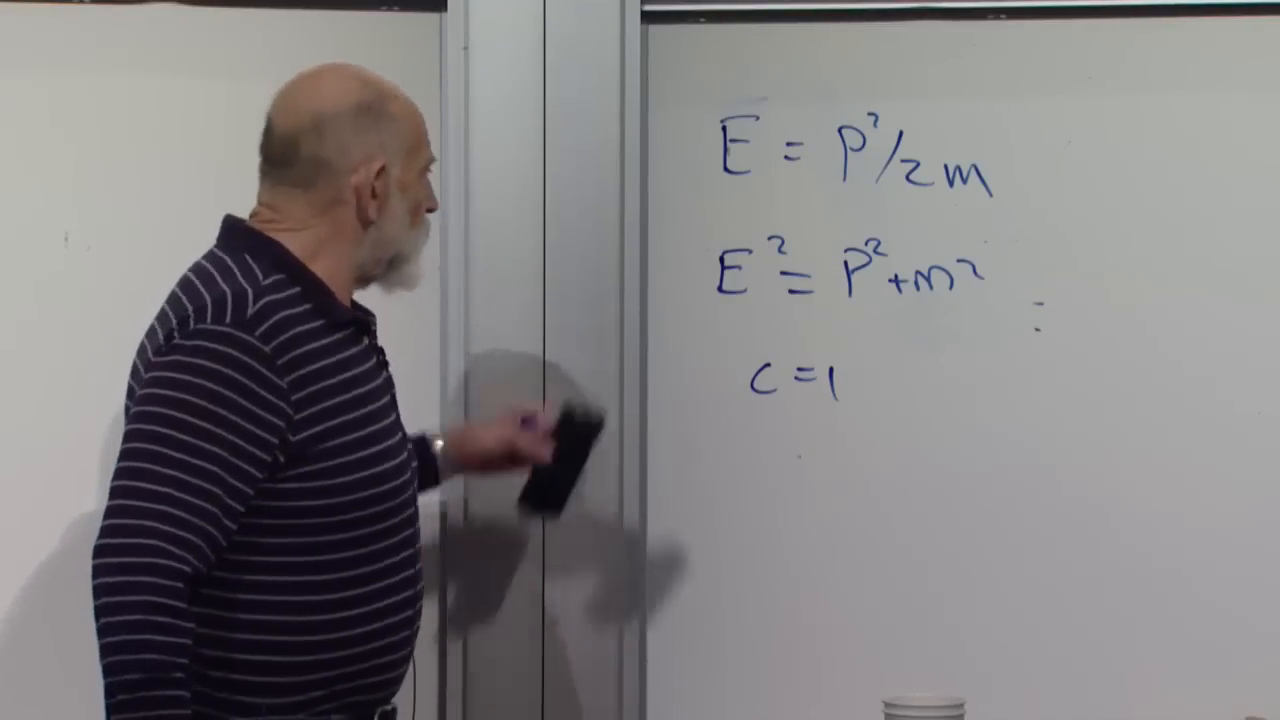
\includegraphics[width=0.94\linewidth]{lecture_09_frame_07.png}
\caption{黑板上从\(E=p^2/2m\)转向相对论关系\(E^2=p^2+m^2\)，其中\(c=1\)。}
\lectureframe{01:10:30}
\end{figure}

将这些替换代入平方后的关系式，得到
\begin{equation}
-\partial_t^2\varphi
=\left(-\partial_x^2+m^2\right)\varphi,
\label{eq:l9-klein-gordon}
\end{equation}
或等价地
\begin{equation}
\left(\partial_t^2-\partial_x^2+m^2\right)\varphi=0.
\end{equation}
这就是克莱因--戈尔登方程。它是一个完全有意义的相对论性场方程，尤其适用于自旋为零的场。但所需的电子方程应当对时间是一阶的，
\begin{equation}
i\partial_t\Psi=H\Psi,
\end{equation}
从而由\(H\)本身，而不仅仅是由\(H^2\)，来生成演化。

人们可以形式地选取
\begin{equation}
H=\sqrt{-\partial_x^2+m^2}.
\end{equation}
这个平方根可以在动量空间中干净地定义，在那里它乘以\(\sqrt{p^2+m^2}\)，但在位置空间中它是一个非局域的伪微分算子。它在技术上有意义，但对于我们所寻求的局域方程而言在美学上无益。因此我们重新开始。

\section{无质量右行波}

首先考虑一个向右运动的无质量粒子。它的正能量和动量满足
\begin{equation}
E=p
\qquad (c=1).
\end{equation}
量子化给出
\begin{equation}
i\partial_t\psi=-i\partial_x\psi,
\end{equation}
或
\begin{equation}
(\partial_t+\partial_x)\psi=0.
\label{eq:l9-right-mover}
\end{equation}
每个解都具有如下形式
\begin{equation}
\psi(x,t)=f(x-t).
\end{equation}
该波形是刚性的，并以光速向右运动。

立刻出现两个困难。第一，如果允许式~\eqref{eq:l9-right-mover}作用于任意的傅里叶模式，那么负动量具有能量\(E=p<0\)，因此哈密顿量没有下界。人为地限制到\(p>0\)只会保留右行者，而这还不是我们想要的电子理论。第二，该方程是一条单行道：它不包含普通的左行电子。我们将首先解决左右问题，而把负能量问题暂时搁置。

\section{两个分量与阿尔法矩阵}

引入两个振幅，
\begin{equation}
\Psi(x,t)=
\begin{pmatrix}
\psi_1(x,t)\\[3pt]
\psi_2(x,t)
\end{pmatrix},
\end{equation}
其中\(\psi_1\)在无质量极限下是右行的，而\(\psi_2\)是左行的：
\begin{align}
(\partial_t+\partial_x)\psi_1&=0,
&
(\partial_t-\partial_x)\psi_2&=0.
\end{align}
量子力学还允许两者的任意叠加。因此一个粒子可以同时具有两个方向的振幅，而不是携带一个一劳永逸地选定的经典标签。

这个额外的二值自由度在代数上类似于自旋，但在一维情形下它不是普通的角动量。定义
\begin{equation}
\alpha=
\begin{pmatrix}
1&0\\
0&-1
\end{pmatrix}
=\sigma_3.
\label{eq:l9-alpha}
\end{equation}
它的\(+1\)本征矢量选出右行分量，而它的\(-1\)本征矢量选出左行分量。在无质量理论中，哈密顿量简单地是
\begin{equation}
H=\alpha p,
\end{equation}
而这两个方程合并为
\begin{equation}
i\partial_t\Psi=-i\alpha\partial_x\Psi.
\label{eq:l9-massless-dirac}
\end{equation}

\begin{classroomqa}
\lecturetimestamp{01:22:44}
\audiencequestion{区分这两个分量的对角矩阵叫什么名字？}
\lecturerresponse{作为泡利矩阵，它是\(\sigma_3\)，而不是\(\sigma_1\)。在狄拉克对当前构造的记号中，我们称它为\(\alpha\)。它的代数就是熟悉的泡利代数，尽管这里的物理标签是方向，而不是自旋角动量。}
\end{classroomqa}

\begin{classroomqa}
\lecturetimestamp{01:23:32}
\audiencequestion{在三维情形下，方向是一个矢量，这个构造是否获得更几何的意义？}
\lecturerresponse{是的。三维问题需要为每个空间方向各用一个矩阵，并导致更丰富的旋量结构。尽管如此，一维模型在其自身的框架内是精确的，并且在没有那种额外复杂性的情况下分离出了本质的左右代数。}
\end{classroomqa}

\begin{figure}[htbp]
\centering
\includegraphics[width=0.94\linewidth]{lecture_09_frame_03.png}
\caption{黑板上的无质量二分量方程：\(H=\alpha P\)，其中对角矩阵为\(\psi_1\)和\(\psi_2\)指定了相反的传播方向。}
\lectureframe{01:26:00}
\end{figure}

单行道问题消失了。负能谱仍然存在，而且我们发现了第三个缺陷：这两个分量仍然是无质量的，并以光速传播。下一步必须引入静止能量并将两个方向耦合起来。

\section{加入质量并发现狄拉克代数}

加入最一般的正比于质量的简单项，
\begin{equation}
H=\alpha p+\beta m,
\label{eq:l9-dirac-hamiltonian}
\end{equation}
其中\(\beta\)只作用于二分量指标。它本来可以是单位矩阵或某个其他矩阵；我们让相对论性色散关系来决定。

由于\(H^2\)必须等于\(p^2+m^2\)，将式~\eqref{eq:l9-dirac-hamiltonian}平方：
\begin{align}
H^2
&=(\alpha p+\beta m)^2\\
&=\alpha^2p^2+\beta^2m^2
+(\alpha\beta+\beta\alpha)pm.
\label{eq:l9-square-dirac}
\end{align}
这些矩阵与\(p\)对易，因为它们作用于内部二分量空间，而\(p\)作用于空间波函数。与式~\eqref{eq:l9-rel-dispersion}相匹配要求
\begin{equation}
\alpha^2=\mathbb{1},
\qquad
\beta^2=\mathbb{1},
\qquad
\{\alpha,\beta\}
=\alpha\beta+\beta\alpha=0.
\label{eq:l9-dirac-algebra}
\end{equation}
第一个条件对\(\alpha=\sigma_3\)已经成立。任何不同的泡利矩阵都与它反对易，并且其平方为单位矩阵。选取
\begin{equation}
\beta=
\begin{pmatrix}
0&1\\
1&0
\end{pmatrix}
=\sigma_1.
\label{eq:l9-beta}
\end{equation}
选取\(\sigma_1\)而不是\(\sigma_2\)是一种基约定；两者在经过幺正基变换后实现相同的代数。

\begin{classroomqa}
\lecturetimestamp{01:33:00}
\audiencequestion{狄拉克只是认识到泡利矩阵满足这些代数条件吗？}
\lecturerresponse{历史上的推导是直接在三维中进行的，并引入了满足所需关系的矩阵。一旦写出这些条件，泡利代数就使一维解变得显而易见：选择两个不同的泡利矩阵。}
\end{classroomqa}

\begin{classroomqa}
\lecturetimestamp{01:34:24}
\audiencequestion{这个\(\beta\)是相对论速度参数\(v/c\)吗？}
\lecturerresponse{不是。它是作用于旋量分量的矩阵。重复使用的字母只是狄拉克的记号；它与运动学量\(v/c\)毫无关系。}
\end{classroomqa}

在三个空间维度中，\(2\times2\)矩阵不足以构成所需反交换矩阵的完整集合。这种扩充被推迟了。在一维中，式~\eqref{eq:l9-alpha}和\eqref{eq:l9-beta}就足够了。

\section{耦合的一维狄拉克方程}

代入\(p=-i\partial_x\)得到哈密顿形式的一维狄拉克方程：
\begin{equation}
i\partial_t\Psi
=\left(-i\alpha\partial_x+\beta m\right)\Psi.
\label{eq:l9-one-dimensional-dirac}
\end{equation}
因为\(\alpha\)是对角的，其导数项使两个分量保持分离。因为\(\beta\)是非对角的，质量项交换它们。逐分量写出，
\begin{align}
i\partial_t\psi_1
&=-i\partial_x\psi_1+m\psi_2,
\label{eq:l9-dirac-component-one}\\
i\partial_t\psi_2
&=+i\partial_x\psi_2+m\psi_1.
\label{eq:l9-dirac-component-two}
\end{align}

\begin{figure}[htbp]
\centering
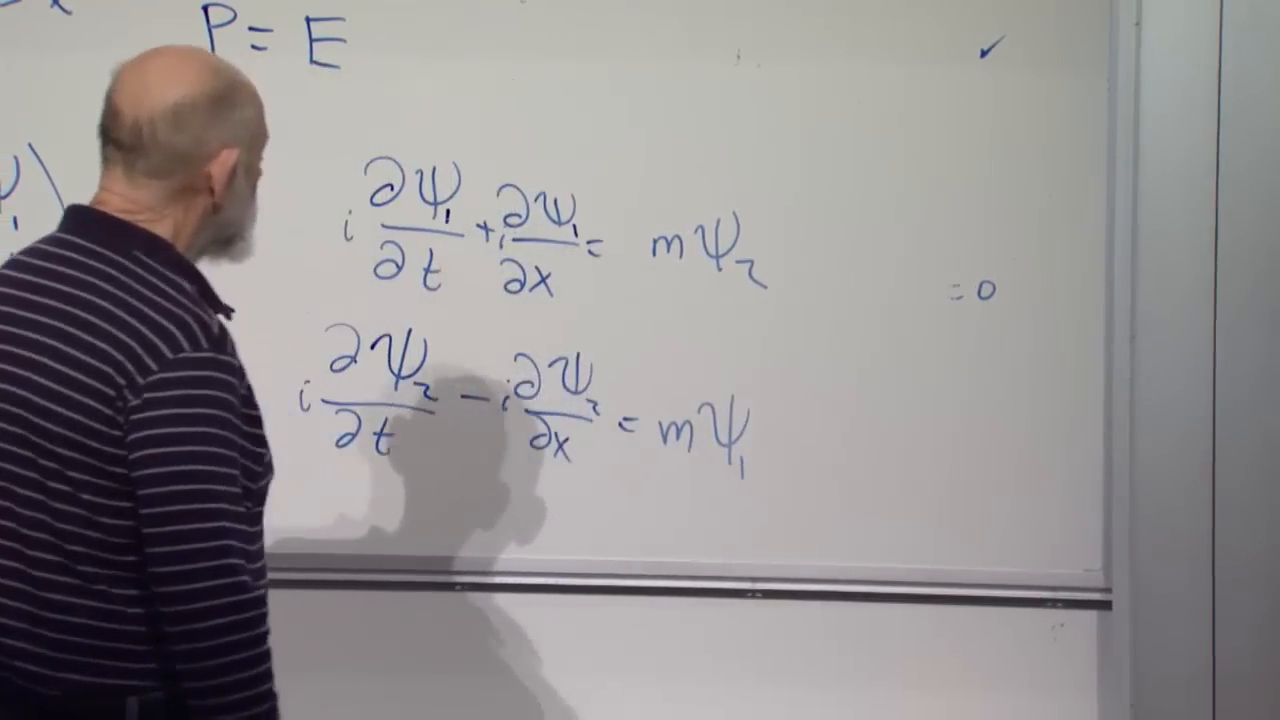
\includegraphics[width=0.94\linewidth]{lecture_09_frame_08.png}
\caption{黑板上的耦合分量方程。相反的导数符号编码了右行和左行运动；非对角质量项交换\(\psi_1\)和\(\psi_2\)。}
\lectureframe{01:37:44}
\end{figure}

一旦\(m\ne0\)，分量就不再独立演化。对一阶方程平方，在每个分量上恢复克莱因--戈尔登算子，
\begin{equation}
\left(\partial_t^2-\partial_x^2+m^2\right)\psi_a=0,
\qquad a=1,2,
\end{equation}
平面波满足\(E^2=p^2+m^2\)。它们的群速度为
\begin{equation}
v_g=\frac{dE}{dp}=\frac{p}{E},
\end{equation}
对于非零质量，其大小小于一。

质量与左右混合之间的关系并非偶然。无质量的右行子在每一次固有洛伦兹助推下都保持为右行子；没有亚光速观察者能追上光并反转其方向。有质量粒子可以被带到静止，然后从沿同一方向运动的更快参考系观察，在那里其速度显得反转了。因此，有质量的相对论理论不能永久保持右和左扇区彼此隔离。非对角质量项恰好提供了所需的耦合。

\begin{classroomqa}
\lecturetimestamp{01:40:01}
\audiencequestion{两个分量的交换是手征振荡吗？}
\lecturerresponse{在这个一维基中，\(\alpha\)区分两个无质量手征方向。质量项是非对角的并混合它们，因此手征性不再守恒。在这个意义上，质量项是手征振荡的来源。}
\end{classroomqa}

\begin{classroomqa}
\lecturetimestamp{01:40:46}
\audiencequestion{为什么费米子方程应该是玻色子方程的平方根？}
\lecturerresponse{不应这样理解。色散关系\(E^2=p^2+m^2\)适用于每个自由相对论粒子，无论统计如何。狄拉克算子恰好提供了克莱因--戈尔登算子的矩阵分解，但这种代数关系并不能从玻色子导出费米子。}
\end{classroomqa}

\begin{classroomqa}
\lecturetimestamp{01:41:31}
\audiencequestion{方程能否简化为分解为独立的左行和右行因子的简单标量分解？}
\lecturerresponse{只有在无质量极限下，两个手征方程才解耦为独立的标量因子。对于\(m\ne0\)，有用的分解是矩阵值的：反交换的\(\alpha\)和\(\beta\)矩阵正是消除不需要的交叉项的东西。}
\end{classroomqa}

\begin{classroomqa}
\lecturetimestamp{01:42:04}
\audiencequestion{这两个耦合方程已经构成狄拉克方程了吗？}
\lecturerresponse{是的。它们合在一起就是一维空间中的狄拉克方程，等价地写成式~\eqref{eq:l9-one-dimensional-dirac}的紧凑形式。通过乘以\(\beta\)可以得到更对称的协变记号，但那种形式被推迟了。}
\end{classroomqa}

有两项任务被有意留待完成。该构造并未消除负能量；它在两个方向扇区中都提供了负能量解，因此这个问题现在更加明显而非更不明显。而且该理论仍然生活在一维空间中。解释负能量解并将矩阵代数扩充到\(3+1\)维是接下来的步骤。
